\documentclass[11pt]{article} %Sets the default text size to 11pt and class to article.
%------------------------Dimensions--------------------------------------------
\topmargin=0.0in %length of margin at the top of the page (1 inch added by default)
\oddsidemargin=0.0in %length of margin on sides for odd pages
\evensidemargin=0in %length of margin on sides for even pages
\textwidth=6.5in %How wide you want your text to be
\marginparwidth=0.5in
\headheight=0pt %1in margins at top and bottom (1 inch is added to this value by default)
\headsep=0pt %Increase to increase white space in between headers and the top of the page
\textheight=9.1in %How tall the text body is allowed to be on each page

\usepackage{hyperref}
\usepackage[usenames,dvipsnames]{color}
\usepackage{paralist}
\usepackage{amsmath}
\usepackage{graphicx}
\usepackage[font=small,labelfont=bf]{caption}
\usepackage{listings}

\lstdefinelanguage{scala}{morekeywords={class,object,trait,extends,with,new,if,while,for,def,val,var,this},
otherkeywords={->,=>},
sensitive=true,
morecomment=[l]{//},
morecomment=[s]{/*}{*/},
morestring=[b]"}
% Default settings for code listings
\lstset{frame=tb,language=scala,aboveskip=3mm,belowskip=3mm,showstringspaces=false,columns=flexible,basicstyle={\small\ttfamily}}

\begin{document}

\title{Analyzing Large Scale Genotype Datasets With \textsc{Gnocchi}}
\author{Frank Austin Nothaft} 
\date{}

\maketitle

\begin{abstract}
The development of inexpensive DNA sequencing technologies has enabled projects
that sequence large cohorts. While many recent projects have tackled the
computationally expensive process of turning raw DNA sequence into genomic
variants, cohort analyses still rely on traditional single node techniques. To
address this problem, we introduce \textsc{Gnocchi}, a Spark SQL based toolkit
for analyzing genomic variants. \textsc{Gnocchi} extends the \textsc{ADAM}
framework for analyzing genomic data with several variation specific patterns,
such as matrix and genotype state views. With \textsc{Gnocchi}, we are able to
parallelize common expensive tasks, such as the training of genome-wide
assocation models, or large scale population stratification.
\end{abstract}

\section{Introduction}
\label{sec:introduction}

Since 2001, improvements in DNA sequencing technologies have allowed the cost of
sequencing a single human genome to drop from \$1 billion to under
\$1,000~\cite{nhgri}. This drastic change in the economics of DNA sequencing
has enabled both the use of sequencing in clinical medicine and the genomic
study of large cohorts. However, this shift brings new problems: the cost of
analyzing genomic data is growing more quickly than the cost of collecting
genomic data is falling. This trend is occurring because the decline in the
cost of sequencing is outpacing Moore's law.

Several recent projects have attempted to cope with the ``DNA data
deluge''~\cite{schatz13} by implementing application programming
interfaces~(APIs) that enable computational biologists to write scalable
algorithms for analyzing DNA sequence data. These projects include
\textsc{Hadoop-BAM}~\cite{niemenmaa12}, a thin layer that allows \textsc{Hadoop}
to read/write genomics file formats; \textsc{BioPig}~\cite{nordberg13} and
\textsc{SeqPig}~\cite{schumacher14}, which present enhancements to the
\textsc{Pig} scripting language for querying genomic data; and
ADAM~\cite{massie13, nothaft15}, a \textsc{Spark}-based API that provides
common genomics query primitives. Additionally, several unpublished projects
are ongoing, such as the ``\textsc{Hellbender}'' rewrite of the Genome Analysis
Toolkit~(\textsc{GATK}, \cite{mckenna10}), the Genomics England
\textsc{OpenCB} project\footnote{\url{https://github.com/opencb/hpg-bigdata}},
and the Google Genomics project\footnote{\url{https://cloud.google.com/genomics/}},
which builds upon \textsc{BigTable}/\textsc{Dremel}~\cite{melnik10} and
\textsc{Spark}.

While these projects have all enabled the use of a scalable analytics system
to analyze genomics data---whether it be \textsc{Apache Hadoop}~\cite{hadoop},
\textsc{Apache Spark}~\cite{zaharia12, zaharia10}, or some other system---these
systems are not optimized for genomic variant data. While genomic variants can
be processed with many of the same patterns as other genomic data types,
genotype data is distinct in that it is most frequently processed using a sparse
matrix-like representation~\cite{layer15, taft14}, or by running a specific
per-site aggregation pattern. In \textsc{Gnocchi}, we build upon the
\textsc{ADAM} project, \textsc{Spark SQL}~\cite{armbrust15}, and recent work
that has added support for common linear algebra operations in \textsc{Apache
Spark}~\cite{zadeh15} to support matrix views of genotype data. Additionally,
we have done preliminary work to optimize the common per-site aggregation
pattern.

In this paper, we describe common kernels that are run across genotype data,
and motivate the need for efficient tools for processing this data in a cluster
environment. With this motivation, we build a modified genotype representation
that is inspired by the \textsc{ADAM}~\cite{nothaft15} schemas and that can map
easily to matrix structures. With this, we demonstrate how multiple common
genotype analysis algorithms can be mapped to this datastructure, and explore
the parallel performance of these algorithms. Although this work is a first
step towards supporting matrix-structured genomics algorithms on top of
\textsc{Spark}, our work illustrates several future steps that will allow for
great improvements in genotype analysis performance.

\section{Background}
\label{sec:background}

Although a single run of a DNA sequencer can produce more than 200 GB of raw
data from an individual whole genome sequencing~(WGS) run, these raw sequences
are not typically directly actionable. Typically, raw DNA sequence data is run
through a variant calling pipeline. Variant calling pipelines statistically
infer the sequence edits between the sample being processed and the reference
genome for their species.  The reference genome represents the ``average'' genome
sequence for a species, as determined from performing a \emph{de novo} assembly
from a pool of individuals. This process estimates both variants and genotypes:
variants are the raw sequence edits, while the genotype is the estimate of how
many copies of each variant the sample has. Once the sequence data has been
transformed into genotype data, it consumes several hundred megabytes~(MB) of
space for a single human genome when stored in a sparse representation, or tens
of gigabytes~(GB) when stored in a dense representation~\cite{danecek11}.

In the case of a single sample, the sparse representation would store genotype
data only at sites where a variant was identified in the sample, while the
dense representation stores data at every site that was sequenced. This dense
representation is used for joint variant calling, which is a process where
observations from multiple samples are pooled in order to improve the accuracy
of the genotype estimation process~\cite{li11}. Once samples from a given cohort
have been merged, the genotypes are typically stored in a semi-sparse
representation where genotypes are stored for all variant where any sample in
the cohort has been observed to have the variant. Statistical tests are run upon
this representation. This representation yields an $n$ by $m$ matrix where $n$
is the number of variants and $m$ is the number of samples in the cohort. We
refer to this representation as semi-sparse as the rows of the matrix are
dense, but the matrix is a sparse representation relative to the $n$ by $g$
matrix that would describe the whole genome ($g$ is the genome size; for a 1,000
sample cohort of humans, $10 m \sim g, g = 3.2$ Giga basepair, Gbp). This data
can be stored in several different ways: the \textsc{VCF} file format stores
rows of the matrix~\cite{danecek11}, while the \textsc{ADAM}~\cite{nothaft15}
and \textsc{GA4GH}\footnote{\url{https://github.com/ga4gh/schemas}, variants of
this schema are used by both the Google Genomics and Genomics England projects.}
schemas store cells of the matrix.

\textsc{Gnocchi} builds these matrix representations on top of the \textsc{ADAM}
project's genotype representation. Specifically, \textsc{Gnocchi} adds the
simplified \texttt{GenotypeState} representation shown in
Figure~\ref{fig:genotype-state}. This representation precomputes the genotype
state from the allelic representation that the \textsc{ADAM} schema uses, and
drops many of the variant calling annotation fields. This representation is
a more compact representation of the genotype at the site and is sufficient for
most statistical analyses. The additional fields included in the \textsc{ADAM}
schema are typically only used for variant quality control analyses, joint
variant calling, and variant filtration. All of these steps are conducted prior
to any large scale statistical tests that are run on the genotypes.

\begin{centering}
\begin{figure}
\begin{minipage}{0.45\linewidth}
\begin{lstlisting}[frame=none]
case class GenotypeState(
  contig: String,
  start: Long,
  end: Long,
  ref: String,
  alt: String,
  sampleId: String,
  genotypeState: Int) {
}
\end{lstlisting}
\end{minipage}
\begin{minipage}{0.45\linewidth}
\begin{verbatim}
record Genotype {
  // core fields
  Variant variant;
  string sampleId;
  boolean splitFromMultiAllelic;
  array<GenotypeAllele> alleles;

  // quality annotations
  VariantCallingAnnotations
    variantCallingAnnotations;

  // estimated likelihoods
  array<float> genotypeLikelihoods;

  // phasing information
  boolean isPhased;
  int phaseSetId;
  int phaseQuality;
}
\end{verbatim}
\end{minipage}
\caption{\textsc{Gnocchi}'s \texttt{GenotypeState} object differs from the
\textsc{ADAM} \texttt{Genotype} object by precomputing the genotype state and by
not including various variant/genotype annotations. The \textsc{ADAM}
\texttt{Genotype} representation included here is abbreviated for clarity.}
\label{fig:genotype-state}
\end{figure}
\end{centering}

There are a variety of statistical algorithms that are run on top of genotype
data. Most of these algorithms are either clustering or regression algorithms.
Clustering algorithms are commonly used to discover population structure in a
large genotyped cohort. For example, the genotype data from the 1,000 Genomes
project~\cite{1kg} comes from 1,092 individuals who represent 26 different
subpopulations. By running principal component analysis~(PCA) on the genotype
data, we can reconstruct the population labels\footnote{\url{http://bdgenomics.org/blog/2015/02/02/scalable-genomes-clustering-with-adam-and-spark/}}.
While this example is not necessarily useful since the population labels were
already known at the start of the study, these sort of clustering/stratification
algorithms are useful when studying populations where the relationships between
individuals is not known \emph{a priori}. This is the case in most large scale
clinical studies.

Regression algorithms are applied to genotype datasets to identify associations
between genomic variants and traits of interest. These tests are commonly known
as genome wide association studies~(GWAS), and they involve the training of
many regression models in parallel. For a study with $n$ genotyped sites and
$p$ phenotypes\footnote{A phenotype is a trait being studied. Commonly, the
phenotype being studied is whether the sample has a disease, or some physical
characteristic~(e.g., height, eye color). Another common form of association
study is an expression quantitative trait locus~(eQTL) test. This test looks for
links between a single variant~(a locus) and the number of copies of a
gene that are created~(expression).}, a GWAS will typically train $np$
orthogonal regression models. Traditionally, these studies have been run using
single machine tools such as PLINK~\cite{purcell07}. While these tools are
widely used in contemporary genomics, they are quite slow\footnote{Recent
benchmarking at \url{https://github.com/jpdna/eQTL-analysis-using-ADAM-and-Spark}
shows that running an eQTL on a 77,000 variant subset of chromosome 22 takes
over 320 minutes on a single machine.}. Recent work~\cite{chang15} has made
improvements to the single thread runtime of these tools, but data ingest
remains a challenge as moderately sized genotype datasets can easily contain
more than one terabyte~(TB) of data. For example, the 1,000 Genomes project
genotype data is 1.6 TB uncompressed. When stored in more efficient formats like
compressed \textsc{VCF}~\cite{danecek11} or \textsc{ADAM}/\textsc{Parquet}, it is
$\mathcal{O}(100\text{GB})$. Since contemporary studies will sequence orders of
magnitude more individuals---the Genomics England project will sequence 100,000
individuals~\cite{uk100k} while the Million Veteran Program~\cite{mvp} has
already genotyped more than 500,000 military veterans---these single node tools
will soon be insufficient.

\section{Implementation}
\label{sec:implementation}

\textsc{Gnocchi} is built upon \textsc{Apache Spark} and the \textsc{ADAM}
genotype schemas~\cite{nothaft15}. \textsc{Gnocchi} uses a mix of the
\textsc{RDD}~\cite{zaharia12} and
\textsc{DataFrame}/\textsc{Dataset}~\cite{armbrust15} APIs. In \textsc{Gnocchi},
we have implemented the following algorithms:

\begin{itemize}
\item ETL/Import:
\begin{enumerate}
\item Squaring of genotype matrix
\item Construction of sparse genotype state matrix from genotype data
\end{enumerate}
\item Clustering:
\begin{enumerate}
\item Wide/flat PCA
\item Sample-sample similarity calculation
\end{enumerate}
\item Regression:
\begin{enumerate}
\item Case-control GWAS
\end{enumerate}
\end{itemize}

Both clustering algorithms are implemented on top of the sparse genotype state
matrix, while the regression algorithms are currently implemented on top of a
squared genotype matrix. This matrix is the semi-sparse/dense row representation
described in~\S\ref{sec:background}.

\subsection{ETL/Import Algorithms}
\label{sec:etl-import}

Our ETL/import algorithms focused on merging genotypes from cohorts into the
matrix structures that are commonly used for analyzing genotype data. The first
algorithm is used to build the semi-sparse/dense row matrix that was described
in~\S\ref{sec:background}, and that is used for regression~(see
\S\ref{sec:regression}). To build this matrix, we first collect a unique list
of the sample identifiers from an \textsc{RDD} of \textsc{ADAM}
\texttt{Genotype}s. We then group all genotypes together by variant. This gives
us an \textsc{RDD} element per variant that has called genotypes. We then
identify which samples are missing genotypes for this variant. Currently, we
just fill these genotypes with a reference call at default ploidy for the
sample. In~\S\ref{sec:future-work}, we describe our future plans for
implementing a more accurate imputation kernel. We simply used this kernel
because the NCI-60 dataset needed a merge function, and since the NCI-60
variant calls were generated from an exome panel, it was reasonable to assume
that all genotyped sites were covered for all samples. This is not necessarily
accurate, but is a reasonable simplifying assumption.

The sparse matrix used for the remaining calculations was generated using the
\textsc{DataFrame}~\cite{armbrust15} API. Since this matrix was intended to
be sparse, we pushed down a predicate to filter out all genotypes that were a
reference call before grouping all genotypes together by variant. We used
the sample identifiers to map samples to integer indices that we used as the
row indices for the sparse matrix. Once genotypes were grouped by position,
we sorted the genotypes by the sample indices and created a distributed
row matrix~\cite{zadeh15}.

\subsection{Clustering}
\label{sec:clustering}

Typically, clustering algorithms that are run on top of genotype datasets on
scalable analytics frameworks do not use all of the genotypes for each sample.
This happens because typically the clustering algorithms that are supported
by systems like \textsc{Spark} are designed to cluster the rows of tall and
skinny datasets. For most genomics applications, we are interested in clustering
along the rows~(the individual samples), but our matrices are wide and flat.
The matrix we described in~\S\ref{sec:etl-import} is a transpose of this
matrix: our columns are our samples, and our rows are our sites. With this
representation, our matrix is now tall and skinny, which allows us to take
advantage of scalable analytics systems. For the sample similarity algorithm,
we are able to natively use the \textsc{DIMSUM} algorithm which is implemented
in \textsc{Spark}~\cite{meng15, zadeh13}. This algorithm efficiently computes
the similarity between two columns of a matrix, and is a natural fit for our
problem.

For PCA, we cannot use the \textsc{Spark} implementation, as it would calculate
the principal components of our transposed matrix. However, we are able to use
\textsc{MLlib}'s singular vector decomposition~(SVD) algorithm to compute PCA.
For a given matrix $A$, SVD decomposes the matrix into three matrices:

\begin{align}
A = U \Sigma V^\text{T}
\end{align}

Due to the unique structure of the SVD~($U$ and $V$ are unitary and $\Sigma$
is diagonal), if $A$ is transposed, yields:

\begin{align}
A^\text{T} = V \Sigma U^\text{T}
\end{align}

Additionally, once we have the SVD, we can compute the principal components
of the original matrix via:

\begin{align}
T_A = U \Sigma
\end{align}

With this, we use the transposed genotype matrix described
in~\S\ref{sec:etl-import}, and calculate the SVD. We then multiply the
$V$ and $\Sigma$ matrices together to recover the PCA of the wide and flat
genotype matrix.

\subsection{Regression}
\label{sec:regression}

While there are a wide assortment of genotype-phenotype association algorithms,
in \textsc{Gnocchi}, we have currently implemented a $\chi^2$ case-control
regression. In this, we take the cross join of all phenotypes and all genotypes
and apply an aggregation function on all of the genotypes to calculate the number
of observed \texttt{(genotype state, phenotype observation)} pairs. Since we are
using a $\chi^2$ test, we can directly apply the test for significance to the
aggregated value. As discussed in~\S\ref{sec:background}, we are working on more
regression kernels, and are evaluating different join materialization
strategies.

\section{Performance}
\label{sec:performance}

We evaluated \textsc{Gnocchi} on data from the NCI-60~(National Cancer
Institute) collection of cancer cell lines~\cite{shankavaram09, reinhold12} and
on data from the 1,000 Genomes project~\cite{1kg}. The NCI-60 dataset was chosen
because it is deeply phenotyped, while the 1,000 Genomes project dataset was
used because it is the largest open access human genotype dataset. Our
evaluation was run on a cluster of 60 machines where each machine was powered
by a 16 core \textsc{Intel E5-2670} running at 2.6 Gigahertz~(GHz), with 256~GB
of memory, and four 3~TB hard disk drives~(HDD). The cluster was running version
5.4.5 of the \textsc{Cloudera Hadoop Distribution}, which corresponds to
\textsc{Apache Hadoop} version 2.6.0. We ran a pre-release build of
\textsc{Apache Spark} 1.6.0, which was built from commit
\texttt{3f4efb5c23b029496b112760fa062ff070c20334}. Data was stored in the
\textsc{Hadoop Distributed File System}~\cite{shvachko10}, which was configured
with a replication factor of two. The nodes in the cluster were connected by a
ten gigabit ethernet switch.

First, we evaluated on the NCI-60 dataset. This dataset is composed of exome
variant calls for 60 different cancer cell lines. Thus, the data is very
sparse~(the exome is $\sim1\%$ of the size of the genome) and fairly small.
In total, it is only 51~MB once compressed. However, the size of the dataset
increases to 164~MB once the variant matrix is squared off. We need to square
off the variant matrix for the NCI-60 dataset because the cell lines were
genotyped individually and not joint called. Once we have squared off the
variant matrix, we can run the GWAS regression kernels. The other analyses
do not require the variants to be semi-sparse/row dense.

The results from the NCI-60 dataset are shown in Figure~\ref{fig:nci-60}. We
ran a scale-out test on our cluster where we scaled the amount of nodes used to
run each kernel from eight nodes to 960 nodes. At each step, we doubled the
number of nodes used, except for the step where we went from 512 nodes to 960
nodes. We were not able to run on 1,024 nodes because several nodes in our
cluster were decommissioned for service. Each node represents a single
\textsc{YARN} container executor; we allocated one processor core and 11~GB
of memory to each executor, along with 3~GB of memory overhead for
\textsc{Spark} off-heap allocation.

\begin{figure}[ht]
\begin{center}
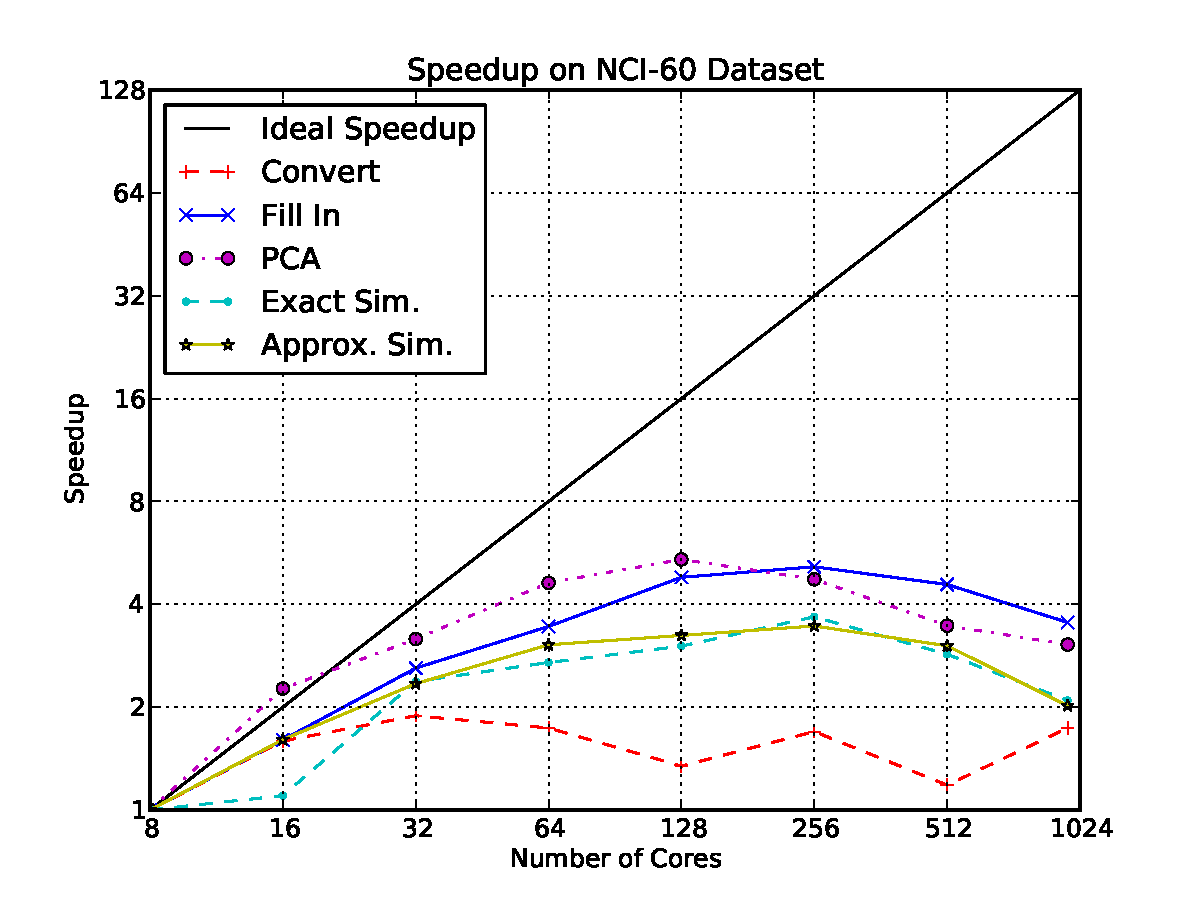
\includegraphics[width=0.75\linewidth]{graphs/speedup_nci-60.pdf}
\end{center}
\caption{Speedup as the number of cores was increased when processing the NCI-60
dataset.}
\label{fig:nci-60}
\end{figure}

On the NCI-60 dataset, we ran all of the kernels we implemented, including
conversion from the legacy \textsc{VCF} file format to the
\textsc{ADAM}/\textsc{Parquet} format. We included the conversion stage because
we needed to manually repartition the input dataset so that we could run our
scalability experiment. We did this because the typical number of input splits
generated when importing the \textsc{VCF} data using
\textsc{Hadoop-BAM}~\cite{niemenmaa12} was 61 partitions, which would limit
our parallelism to 61 executors. This import stage did not parallelize well,
as the conversion from \textsc{VCF} to the \textsc{ADAM} schema would run on
61 executors, followed by a stage where the records would be redistributed
to more executors via a shuffle. For our experiment, we repartitioned our data
so that we had two partitions per executor for load balance. Beyond the
conversion step whose performance was approximately constant for all cluster
sizes, most of our algorithms would scale through 128--256 nodes. Specifically,
the performance of PCA peaked at 128 nodes, while all other algorithms peaked
at 256 nodes. Exact runtimes are listed in Table~\ref{tab:nci-60}. These
runtimes excluded \textsc{YARN} job submission and scheduling delay.

\begin{table}[ht]
\centering
\caption{Performance Summary for NCI-60}
\label{tab:nci-60}
\begin{tabular}{ l | c c c | c }
\bf Tool & \bf Single Runtime (sec) & \bf Fastest Runtime (sec) & \bf Speedup & \bf Cores \\
\hline
\hline
Fill In & 154.0 & 29.9 & $5.15\times$ & 256 \\
PCA & 117.5 & 21.7 & $5.45\times$ & 128 \\
Exact Sim. & 90.8 & 24.8 & $3.66\times$ & 256 \\
Approx. Sim. & 89.5 & 25.9 & $3.45\times$ & 256 \\
\end{tabular}
\end{table}

We ran an additional speedup experiment using the 1,000 Genomes~\cite{1kg}
dataset. The 1,000 Genomes genotype dataset is 49~GB when converted to
\textsc{ADAM}/\textsc{Parquet}, and is 1.1~TB when stored as uncompressed
\textsc{VCF}. We were only able to run the approximate sample similarity kernel
on this dataset. We were only able to run this because there is a regression
in \textsc{Spark} 1.6 that caused buffer underflows when processing this data
with the \textsc{DataFrame} API. Because of this, we fell back on code that we
had written originally against the \textsc{RDD} API. Because of this, we ran
these experiments with the \textsc{Spark} 1.3.0 stable release that ships with
\textsc{CDH} 5.4.5.

\begin{figure}[ht]
\begin{center}
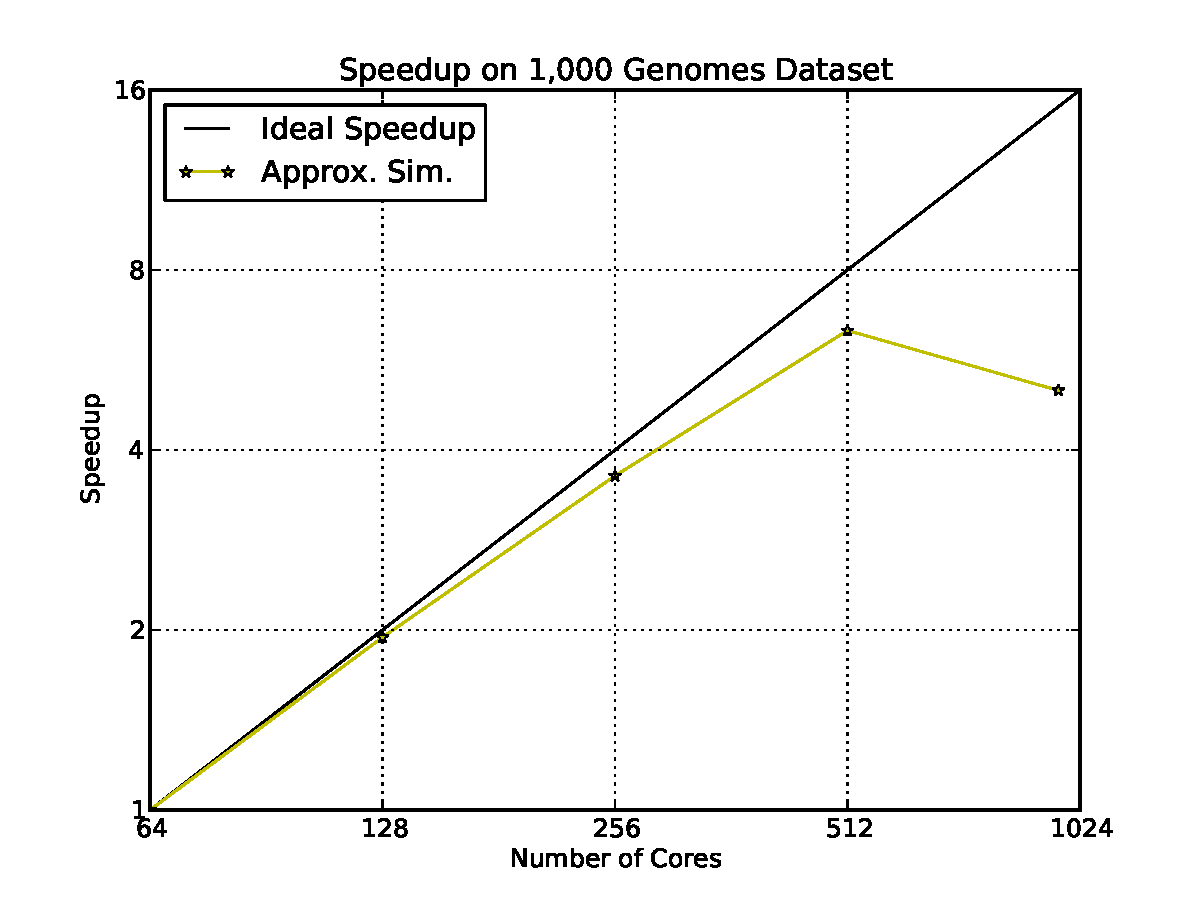
\includegraphics[width=0.75\linewidth]{graphs/speedup_1kg.pdf}
\end{center}
\caption{Speedup as the number of cores was increased when processing the 1,000
Genomes dataset.}
\label{fig:1kg}
\end{figure}

In this experiment, we forced the input dataset to be repartitioned into 4,096
partitions. This represents four partitions per core when running on a 1,024
executor cluster. Performance peaked at 512 nodes. We did not see a speedup when
moving between 512 and 960 nodes for two reasons. First, running with all 960
executors repeatedly caused task failures that did not reproduce on smaller
clusters. Although we repeated the experiment multiple times on 960 cores, the
errors persisted across all runs. We believe that this may either be due to a
hardware or configuration problem in the cluster. Additionally, since the
cluster is running as 960 cores instead of the full 1,024 core configuration,
there was not an even distribution of tasks across executors. Since
\textsc{Spark} is built around a bulk synchronous parallel~\cite{zaharia12}
scheduling abstraction, we must block the cluster until all tasks in a single
stage complete. This is an artifact of our current cluster configuration, as
several nodes have been temporarily decommissioned for service.

\section{Future Work}
\label{sec:future-work}

This paper presents preliminary work on the \textsc{Gnocchi} project. We are
currently working on an enhanced imputation kernel that makes use of sample
similarities to infer genotypes at a site. Currently, our kernel is general,
but we plan to use a PCA based approach. Additionally, we are working on more
clustering algorithms~(specifically, a wide-and-flat $k$-means implementation),
and the implementation of linear and logistic regression for genotype-phenotype
association. These two regression kernels will add support for covariates.

One of the more interesting optimizations that we are looking at targets the
cross join that is executed as part of a genotype-phenotype regression~(see
\S\ref{sec:regression}). In our experiments, we tested on a moderately deeply
phenotyped population~($\mathcal{O}(10)$ phenotypes) across a small set of
genotypes. As such, the duplication of data created by this cross join was
not a big problem. However, for larger analyses---such as large scale eQTL
tests with $\mathcal{O}(10,000)$ phenotypes---this cross join is unrealistic.
As future work, we plan to evaluate strategies that push the cross join into
the aggregation kernel. While this requires repeatedly computing the join,
we believe that this join is fairly inexpensive.

\section{Conclusion}
\label{sec:conclusion}

In this paper, we have demonstrated the \textsc{Gnocchi} framework for parallel
genotype analysis. \textsc{Gnocchi} is implemented on top of \textsc{Apache
Spark}'s \textsc{RDD}~\cite{zaharia12, zaharia10} and
\textsc{DataFrame}/\textsc{Dataset}~\cite{armbrust15} APIs, as well as the
\textsc{ADAM}~\cite{massie13, nothaft15} schemas. With \textsc{Gnocchi}, we have
demonstrated how the analysis of genotype datasets can be scaled to hundreds
of cores. \textsc{Gnocchi} is open source software released under an\textsc{
Apache 2} license,\footnote{\url{http://www.apache.org/licenses/LICENSE-2.0}}
and can be downloaded from \url{https://github.com/fnothaft/gnocchi}.

\bibliographystyle{acm}
\bibliography{fnothaft-gnocchi-cs294}

\end{document}
